\documentclass{article}

\usepackage[final]{corl_2026}
\usepackage{graphicx}
\usepackage{booktabs}
\usepackage{amsmath}
\usepackage{array}
\usepackage{url}
\setlength{\textfloatsep}{6pt}
\setlength{\floatsep}{6pt}
\setlength{\intextsep}{6pt}

\title{Reward Shaping and Curriculum PPO for Sparse-Reward SoccerTwos Control}
\raggedbottom

\author{
  Vedaang Chopra\\
  Georgia Institute of Technology\\
  United States\\
  \texttt{vedaangchopra@gatech.edu}
  \And
  Manya Jain\\
  Georgia Institute of Technology\\
  United States\\
  \texttt{manyajain@gatech.edu}
}

\begin{document}
\maketitle

\begin{abstract}
  Our project studies PPO-based policy learning in SoccerTwos, a sparse-reward Unity soccer environment where agents must learn to reach the ball, move it towards goal and score using limited feedback. We examined two changes to a basic PPO baseline that was learning slowly. Firstly, curriculum learning with progressively harder start states. Then, reward shaping with small, dense bonuses for ball-directed progress. Curriculum training yielded the strongest policy, while reward shaping enhanced early training from 0.2399 to 0.4036 mean episode reward at an identical 2M-step budget. After about 30 million environment steps, the final curriculum v3 agent, exported as \texttt{TEAMNAME\_v3\_AGENT}, achieved a final mean episode reward of 1.9692. It also won eight out of ten recorded matches against the PPO baseline. These findings imply that curriculum learning was the best approach to overcome the primary bottleneck, which was sparse-reward exploration.
\end{abstract}

% \keywords{Reinforcement Learning, SoccerTwos, Curriculum Learning}
\section{Overview}

In the 2-team Unity soccer game SoccerTwos, cube agents must interact to learn
how to move, approach the ball, defend and score goals. The default reward is
sparse making the task difficult because until the agent achieves significant
soccer events like scoring or conceding, many trajectories include little
helpful feedback. Because PPO is stable and popular for continuous interaction
contexts, and supported by the RLlib training pipeline implemented in the
project, we approached this as a policy-learning issue and chose it as the
basis method. The primary objective was find out if PPO might learn better
soccer behavior with more structure. Because of this, we compared a
sparse-reward PPO baseline, a reward-shaped PPO agent with dense progress
signals, and a curriculum PPO agent that starts from easier states before
training on harder game situations. The final submitted policy,
\texttt{TEAMNAME\_v3\_AGENT}, was given by extending the best curriculum PPO
checkpoint to a longer training budget.

% \begin{figure}[t]
%     \centering
%     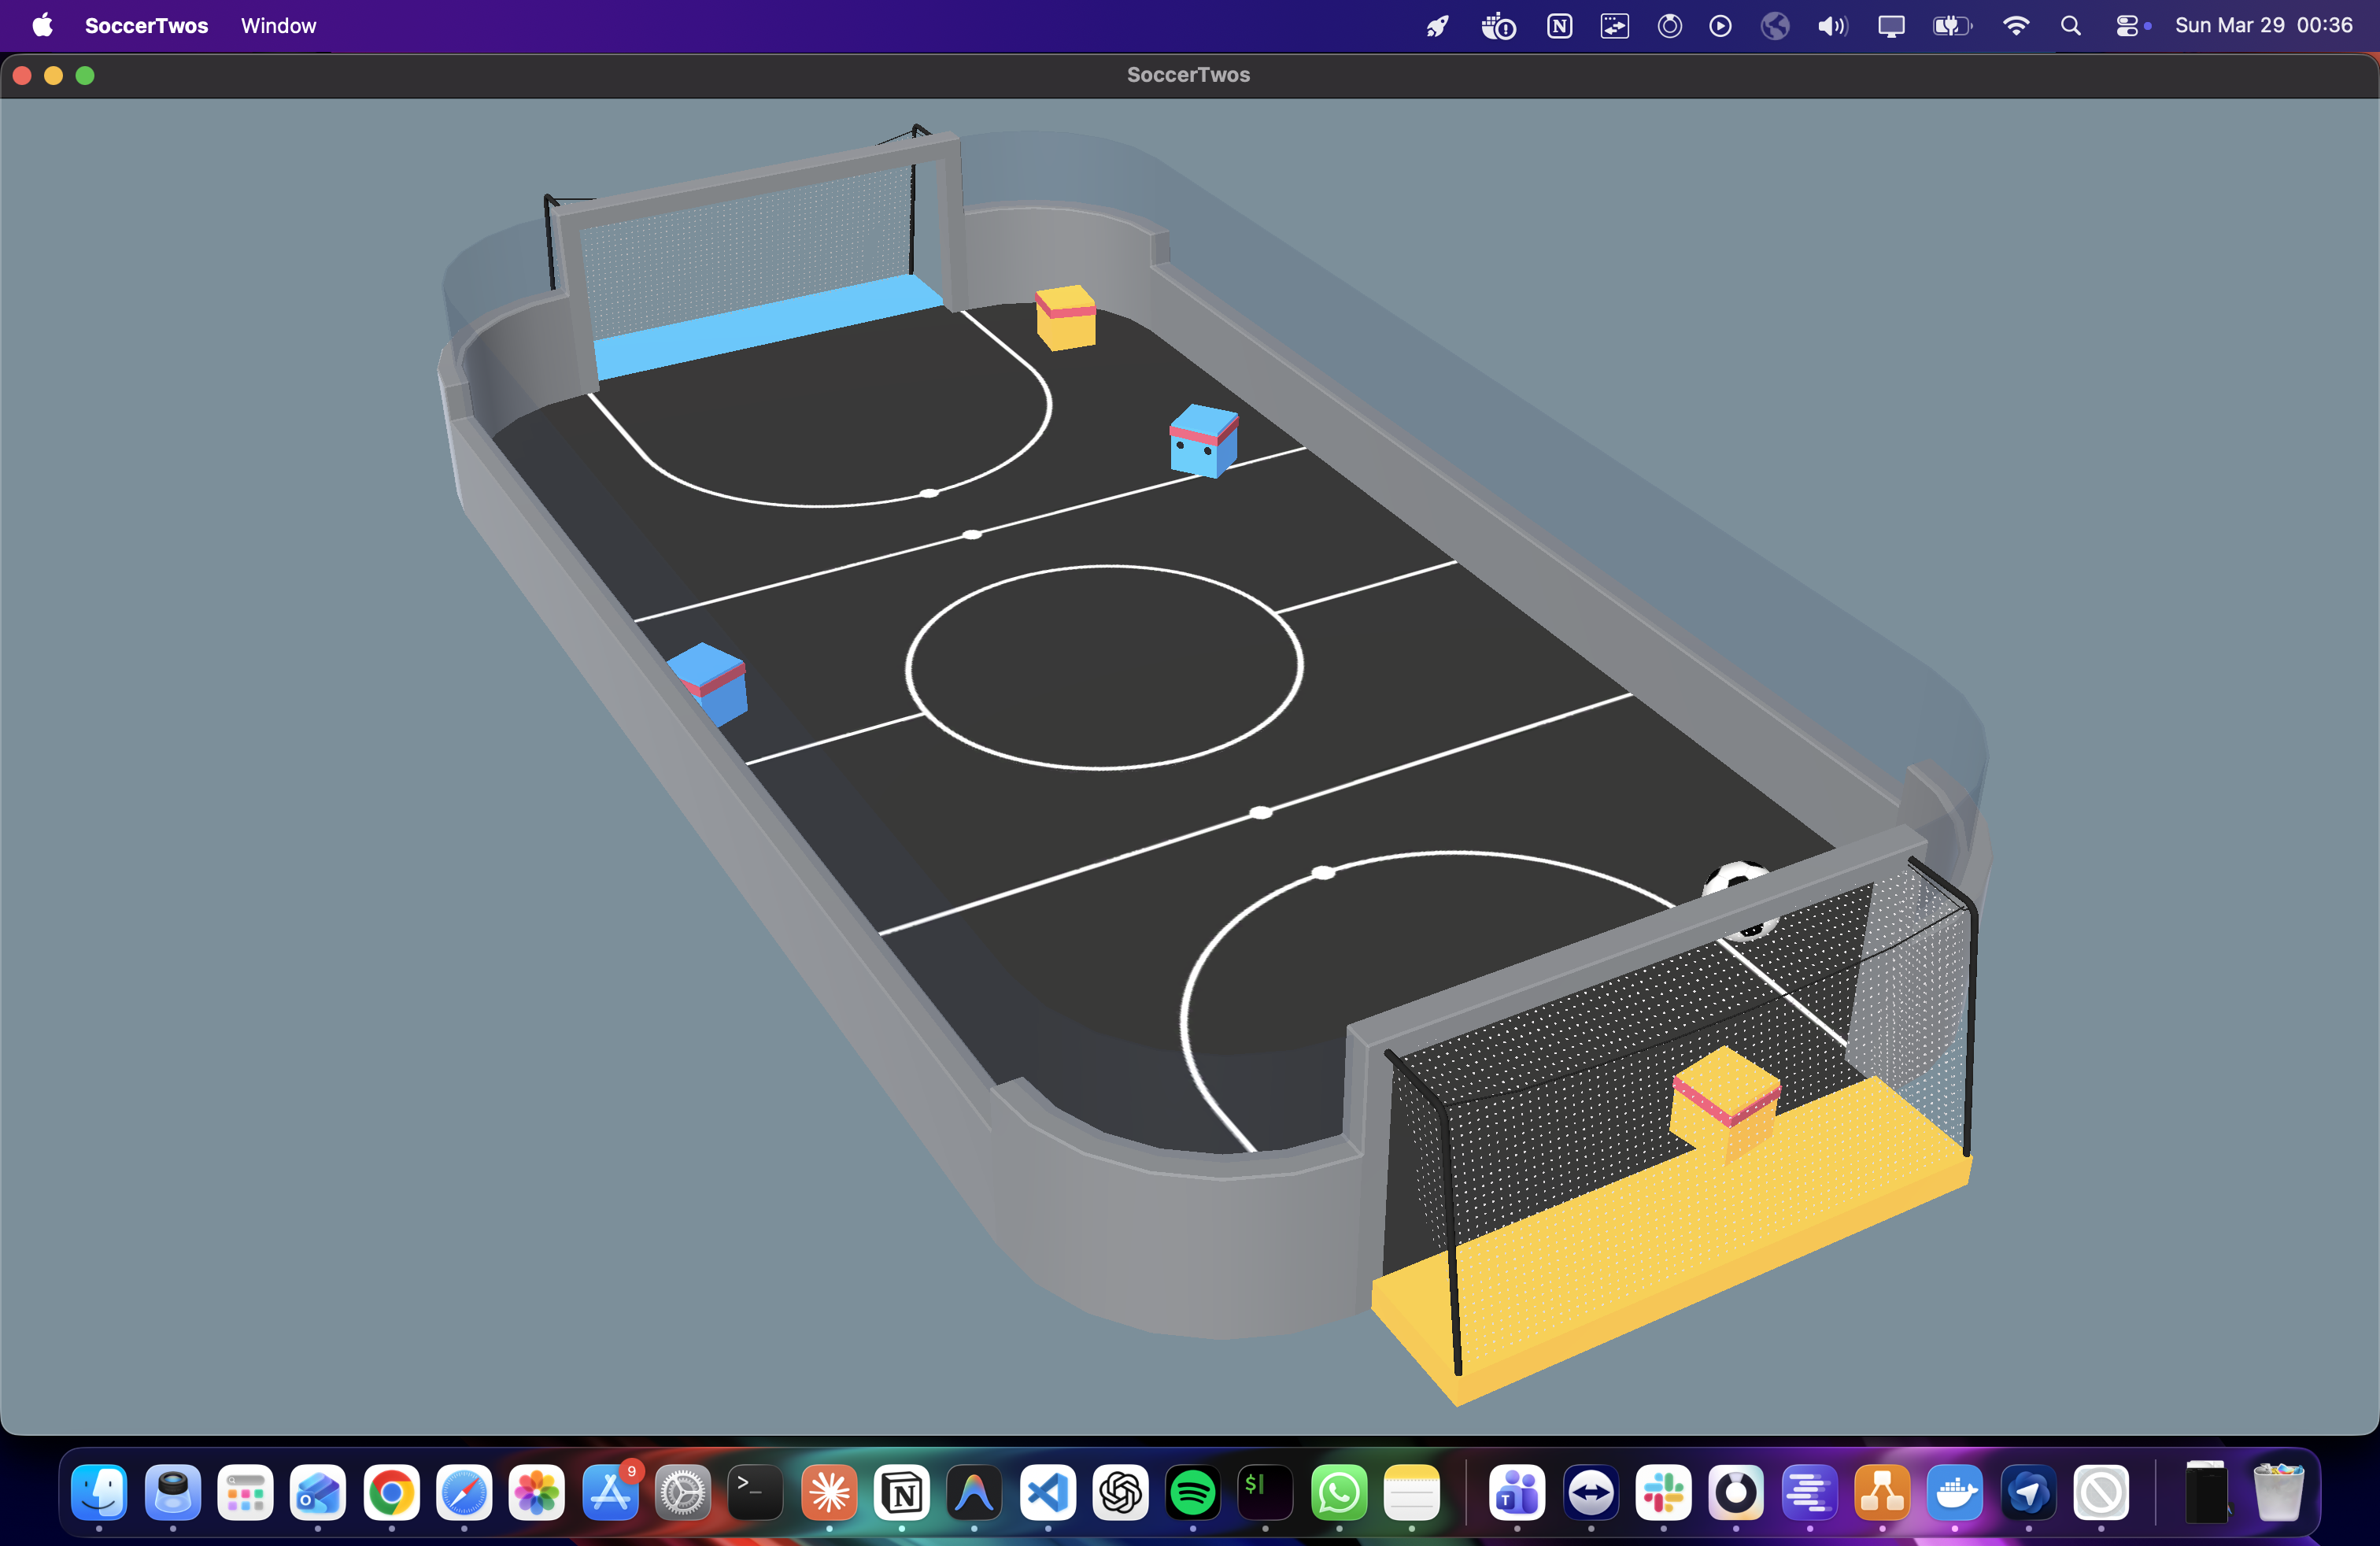
\includegraphics[width=0.65\linewidth]{figures/envt.png}
%     \caption{SoccerTwos environment used for training and evaluation. The task requires cube agents to move in the arena, interact with the ball, and score in the opponent goal.}
%     \label{fig:env_screenshot}
% \end{figure}

% \section{Method Description}

% \textbf{PPO baseline.}
% The baseline policy-gradient approach we employed was Proximal Policy Optimization (PPO). A feed-forward ReLU actor-critic network and the default sparse SoccerTwos reward were used to train the baseline agent. Because we know that PPO limits policy updates through a clipped objective, it was a sensible place to start. This is because it helps avoid big and unstable adjustments from rollout data. The policy/value model employed a single 512-width hidden layer with shared value layers in the baseline and reward-shaped runs.

% \textbf{Reward-shaped PPO.}
% Because there are sparse rewards in the SoccerTwos task, an agent may move for a lot of steps without obtaining a clear indication and feedback of whether it is approaching useful soccer behavior. We wrapped up the training environment with a shaping term that was calculated from the environment \texttt{info} dictionary in order to lower this exploration strain. Let $d_{pb}$ denote the player-to-ball distance and $d_{bg}$ show the ball-to-goal distance. At every transition, the wrapper adds
% \[
% r_{\mathrm{shape}} =
% \mathrm{clip}\left(0.01(d_{pb}^{t-1}-d_{pb}^{t}) +
% 0.02(d_{bg}^{t-1}-d_{bg}^{t}), -0.05, 0.05\right).
% \]
% When the controlled player approaches the ball or the ball approaches the opponent's goal, this provides a small positive bonus. The shaped signal directs exploration without replacing the primary task objective since the clipping keeps the shaping reward limited elative to actual scoring outcomes. The exported policy does not need privileged \texttt{info} fields at inference time. This shape is only utilized during training. For sparse-reward RL~\citep{ng1999policy}, this design adheres to the overall motivation of reward shaping.

% \textbf{Curriculum PPO.}
% Curriculum learning was our second modification. The curriculum starts the agent in simpler scenarios and progressively raises the complexity rather than training from the entire difficult game distribution right away. When the running \texttt{episode\_reward\_mean} is more than 1.5, a callback sets the starting ball and player states using the Unity environment channel and moves through 5 tasks. This goes from “Very Easy Goal” to “Random Players. Because the agent initially learns simple ball-to-goal behavior and then applies that behavior to increasingly difficult starting situations, early exploration is more productive. A deeper ReLU MLP with shared value layers and hidden layers \([256,256]\) was also employed in the curriculum policy. The final v3 policy resumed the strongest curriculum checkpoint. It also extended training to about 30.0M environment steps, following the curriculum-learning idea that we learned that easier early tasks can improve learning in sparse-reward settings~\citep{bengio2009curriculum}.

\section{Method Description}

\textbf{PPO baseline.}
The baseline used RLlib PPO with the default sparse SoccerTwos reward and a feed-forward ReLU actor-critic network. PPO was chosen because its clipped objective limits destructive policy updates from rollout data. The baseline and reward-shaped agents used a shared policy/value model with one 512-unit hidden layer.

\textbf{Reward-shaped PPO.}
To reduce sparse-reward exploration difficulty, the shaped agent added a small training-only reward from the environment \texttt{info} dictionary. Let $d_{pb}$ be player-to-ball distance and $d_{bg}$ be ball-to-goal distance. At each transition,
\[
  r_{\mathrm{shape}} =
  \mathrm{clip}\left(0.01(d_{pb}^{t-1}-d_{pb}^{t}) +
  0.02(d_{bg}^{t-1}-d_{bg}^{t}), -0.05, 0.05\right).
\]
This rewards moving toward the ball and moving the ball toward the opponent
goal, while clipping keeps the bonus small relative to scoring rewards. The
exported policy does not use privileged \texttt{info} fields at inference time.
This follows the usual motivation for reward shaping in sparse-reward
RL~\citep{ng1999policy}.

\textbf{Curriculum PPO.}
The curriculum agent changed the training distribution by starting from easy game states and gradually increasing difficulty. A callback set initial ball and player states through the Unity environment channel and advanced through five tasks, from ``Very Easy Goal'' to ``Random Players,'' once \texttt{episode\_reward\_mean} exceeded 1.5. The curriculum policy used a shared-value ReLU MLP with hidden layers \([256,256]\). The final v3 policy resumed the strongest curriculum checkpoint and trained for about 30.0M steps so the agent could stabilize on later randomized stages after learning easier early tasks~\citep{bengio2009curriculum}.

\textbf{Final hyperparameters.}
Our submitted policy was trained with Ray RLlib PPO using the PyTorch backend. In the final v3 run, we used a learning rate of \(5\times10^{-5}\) and discount factor \(\gamma=0.99\). We also used PPO clipping parameter 0.3, 30 SGD epochs per update, and train batch size 80,000. Others included minibatch size 8,000, rollout fragment length 2,000, gradient clipping at 0.5, 40 rollout workers, and 1 GPU. The exported submission package was \texttt{TEAMNAME\_v3\_AGENT}.

\begin{table}[t]
  \centering
  \small
  \caption{Main PPO training configurations used in the project.}
  \label{tab:methods}
  \begin{tabular}{lccc}
    \toprule
    Method            & Reward                    & Curriculum & Network    \\
    \midrule
    PPO baseline      & sparse                    & no         & [512]      \\
    Reward-shaped PPO & sparse + shaping          & no         & [512]      \\
    Curriculum PPO    & sparse + curriculum setup & yes        & [256, 256] \\
    Curriculum PPO v3 & resumed curriculum        & yes        & [256, 256] \\
    \bottomrule
  \end{tabular}
\end{table}

\section{Preliminary Results}

Figure~\ref{fig:curves} shows the main training comparison. Plain PPO struggled
with the sparse reward, reaching only 0.2399 mean episode reward after 2.0M
steps. Reward shaping improved this to 0.4036 at the same budget, but the
largest gain came from curriculum learning. The first curriculum run reached
1.7869 mean reward after 2.06M steps, and the extended curriculum v3 run
reached 1.9692 final mean reward, with a best logged value of 1.9705 at 29.85M
steps. These curves suggest that curriculum design was more important than
reward shaping alone for learning useful SoccerTwos behavior.

\begin{figure}[htbp]
  \centering
  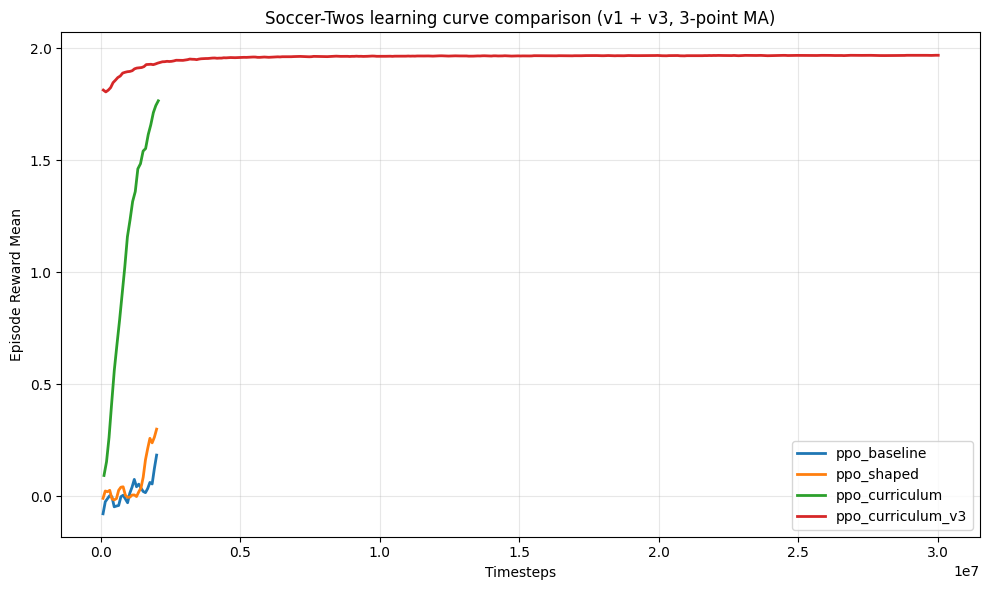
\includegraphics[width=0.75\linewidth]{figures/all_comparison.png}
  \caption{Mean episode reward over training for baseline PPO, reward-shaped PPO, curriculum PPO, and the extended curriculum v3 policy. Reward shaping improves over the sparse-reward baseline, but curriculum training gives the largest gain.}
  \label{fig:curves}
\end{figure}

Table~\ref{tab:eval} reports the recorded headless evaluation matches for the
final curriculum v3 policy. Because the number of evaluation episodes is small,
these results should be treated as preliminary rather than definitive. Still,
the v3 policy won 8 of 10 matches against the PPO baseline and 6 of 10 matches
against the earlier curriculum policy, which is consistent with the
learning-curve improvement.

\begin{table}[t]
  \centering
  \small
  \caption{Recorded headless evaluation summaries for the final curriculum v3 policy. Match counts are small, so these results are preliminary.}
  \label{tab:eval}
  \begin{tabular}{lrrrr}
    \toprule
    Matchup                      & Episodes & Wins & Agent mean & Opponent mean \\
    \midrule
    Curriculum v3 vs. baseline   & 10       & 8    & 1.1140     & -1.2084       \\
    Curriculum v3 vs. curriculum & 10       & 6    & 0.3407     & -0.4258       \\
    \bottomrule
  \end{tabular}
\end{table}

\begin{figure}[htbp]
  \centering
  \begin{minipage}[t]{0.45\linewidth}
    \centering
    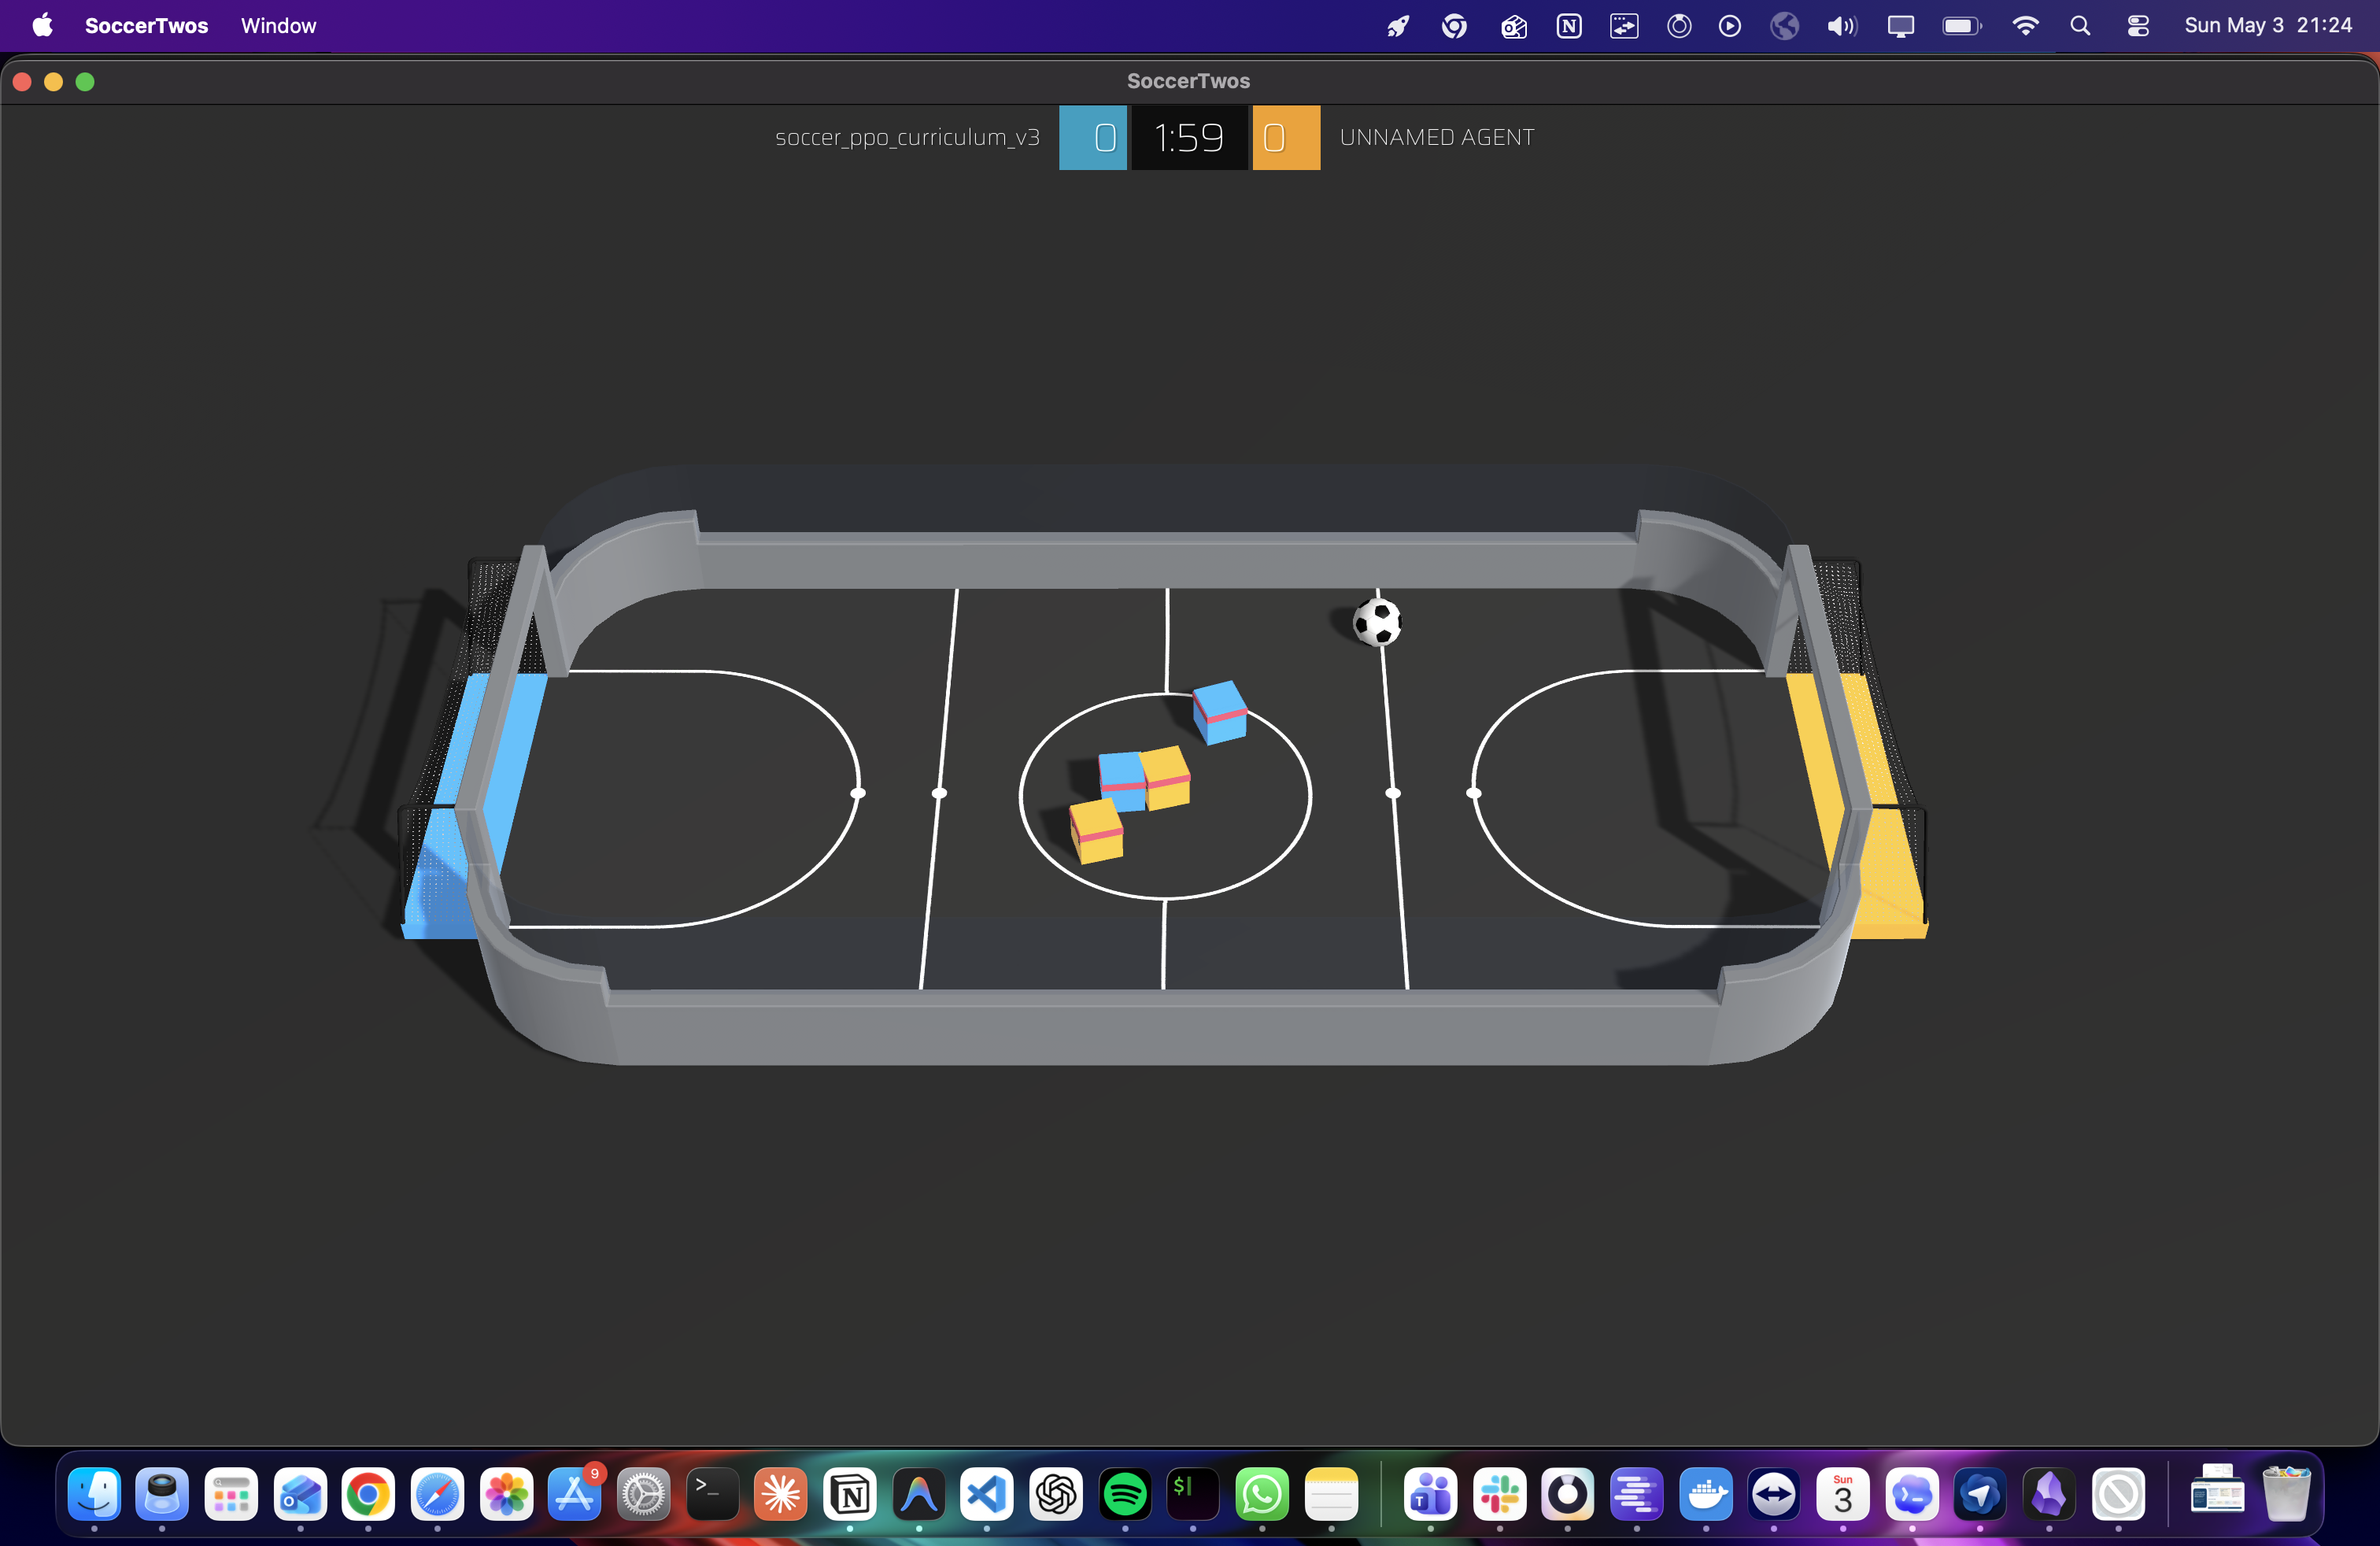
\includegraphics[width=\linewidth]{figures/figure-gameplay-1.png}
  \end{minipage}
  \hfill
  \begin{minipage}[t]{0.45\linewidth}
    \centering
    
\includegraphics[width=\linewidth]{figures/fig-gameplay-2.png}
  \end{minipage}
  \caption{Gameplay screenshots from the final \texttt{TEAMNAME\_v3\_AGENT} evaluated in the SoccerTwos environment. The agent (blue team) consistently moves toward the ball and positions itself to score.}
  \label{fig:gameplay}
\end{figure}

Figure~\ref{fig:v3_diagnostics} shows the detailed training diagnostics for the
final curriculum v3 run. The mean episode reward quickly approached 2.0 and
remained stable, while episode length dropped sharply and then stabilized. This
suggests that the final policy learned to reach terminal soccer outcomes more
efficiently. The PPO diagnostics also show decreasing entropy and value loss,
which is consistent with the policy becoming less random and the critic fitting
the return signal more accurately.

\begin{figure}[htbp]
  \centering
  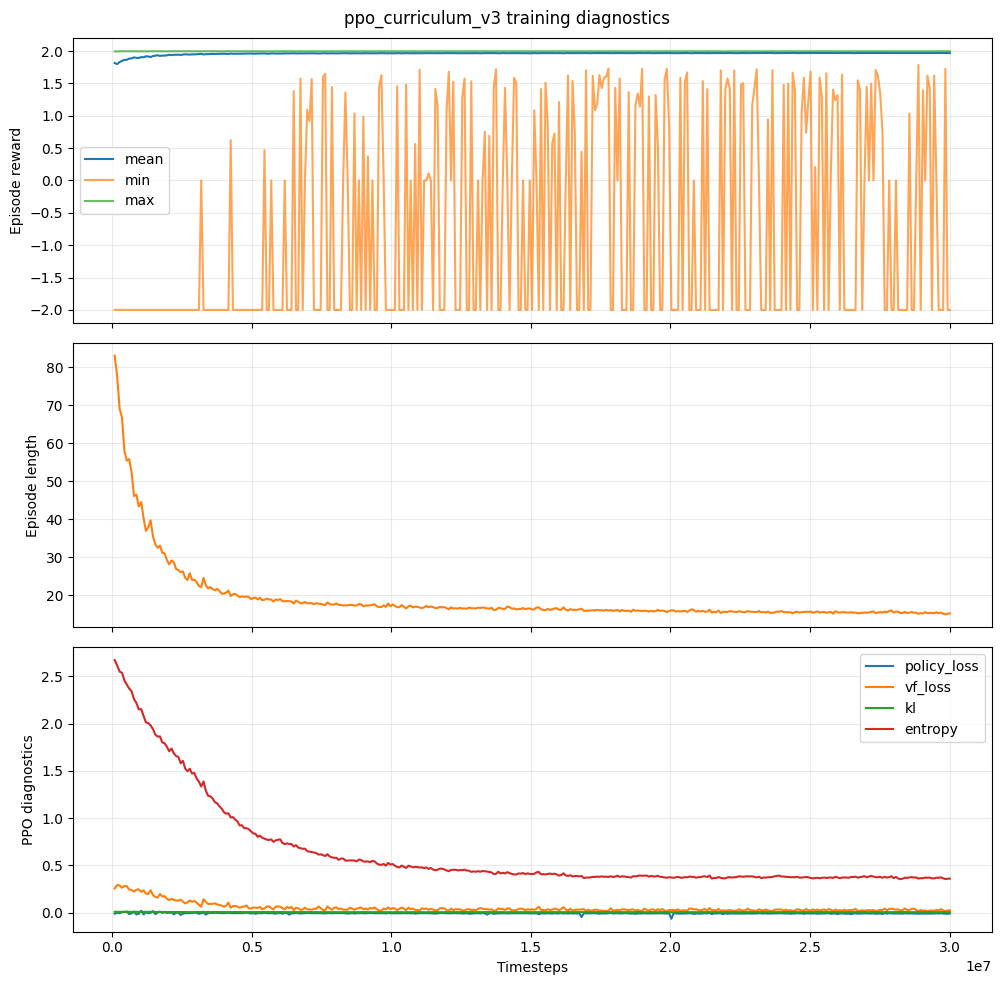
\includegraphics[width=0.75\linewidth]{figures/best_rl_algo.png}
  \caption{Detailed diagnostics for the final \texttt{ppo\_curriculum\_v3} run. Mean reward stabilizes near 2.0, episode length decreases substantially, and PPO diagnostics show stable convergence behavior.}
  \label{fig:v3_diagnostics}
\end{figure}

\section{Reward, Observation, and Architecture Modifications}

\textbf{Reward modification.}
The main reward-level change is the training-only \texttt{RewardShapingWrapper}. It uses \texttt{player\_info} and \texttt{ball\_info} to reward progress toward the ball and ball progress toward the opponent goal. The shaping bonus is clipped to \(\pm 0.05\) and added only during training, so the exported policy does not require privileged \texttt{info} fields. This improved the 2.0M-step mean reward from 0.2399 for baseline PPO to 0.4036 for reward-shaped PPO, helping early exploration but not producing the strongest final policy.

\textbf{Observation and action handling.}
No custom observation-space wrapper or Unity-side observation rewrite was used. The policy uses the provided 336-dimensional SoccerTwos observation vector. The main interface adaptation is action handling: training uses flattened \texttt{Discrete(27)} actions, while live matches use branched \texttt{MultiDiscrete([3,3,3])} actions. Therefore, this report does not claim an observation modification.

\textbf{Architecture and curriculum modification.}
The baseline and reward-shaped PPO agents use one 512-unit hidden layer, while the curriculum PPO agents use a two-layer \([256,256]\) ReLU MLP with shared value layers. Curriculum training also changes the initial-state distribution, starting with easier near-goal situations before progressing to harder ball and player placements. This was the most effective modification, producing much higher training rewards and better recorded match outcomes than baseline PPO.

% \section{Limitations and Future Work}
% Evaluation size was our primary limitation. The match results should be regarded as preliminary because the strongest recorded comparison against the PPO baseline consists of 10 headless episodes rather than a broader 100-episode evaluation. Additionally, the final agent should not be understood as having learned complete multi-agent coordination. This includes passing or team positioning. This is because training was conducted in a simplified single-player situation against a predefined opponent policy. We also noticed that although it was investigated as an alternative approach, imitation learning was not the ultimate successful strategy. Based on these, we think that future research should evaluate reward-shaped PPO directly against curriculum v3 in head-to-head matches. It should also conduct bigger evaluations versus random, baseline, and TA agents. Lastly, it should examine if the curriculum policy stands against stronger multi-agent opponents or self-play.

\section{Limitations and Future Work}
The main limitation is evaluation size. The strongest recorded comparison
against the PPO baseline used only 10 headless episodes rather than a larger
100-episode evaluation, so the match results should be treated as preliminary.
Training was also done in a simplified single-player setting against a fixed
opponent, so the final policy should not be interpreted as learning full
multi-agent coordination such as passing or team positioning. Imitation
learning was explored, but it was not part of the final successful method.
Future work should run larger evaluations against random, baseline, and TA
agents; compare reward-shaped PPO directly against curriculum v3; and test
whether the curriculum policy remains robust under self-play or stronger
multi-agent opponents.

\section{GitHub Link and Acknowledgments}
\url{https://github.com/Vedaang-Chopra/RL_Soccer_project}

We used ChatGPT~\citep{openai2026chatgpt} and Gemini~\citep{google2026gemini}
for feedback, editing suggestions, code editing, bug fixing, formatting, brainstorming and \LaTeX{} cleanup. All experiments, implementation choices, reported results,and final claims are the authors' original work.

\bibliography{example}

\end{document}
